\section{Pain}
Pain is defined, by the International Association for the Study of Pain (IASP), as an unpleasant sensory and emotional experience associated with actual or potential tissue damage \cite{(Marsky and Bogduk, 1994}. Pain is a sudden or slow onset of any intensity from mild to severe pain~\cite{Mello2016} and can categorized based on the pain experience as acute, chronic and intermittent pain~\cite{Goldberg2011}. Acute pain is anticipated or predictable, while  chronic pain is not anticipated or predictable. Chronic pain has a duration greater than three months with a constant or recurring of pain ~\cite{Mello2016}. 

Pain is a worldwide problem and affects all populations regardless of gender, age, income, ethnicity or geography, but the distribution across the globe differs\cite{Goldberg2011}. 
The prevalence and incidence is high despite the complexity of quantifying pain\cite{Goldberg2011}. It is estimated that 20\% of the world's populations adults suffer from pain and each year 10 \% is diagnosed with chronic pain~\cite{Goldberg2011}. 

The frequently causes of pain are operations, cancer, osteoand rheumatoid arthritis, injuries and spinal cord problems~\cite{Goldberg2011}. Furthermore, pain can causes to different sequelae, such as depression, inability to work, limit social relationships and suicidal thoughts\cite{Goldberg2011}. 

People with chronic pain often complain of cognitive problems which interfere with their daily functions~\cite{Geisser2018}. Additionally, it is indicated that among people with chronic pain there is a consistent evidence for disturbances in attentional capacity, processing speed, and psychomotor speed~\cite{Geisser2018}. However, the relationship between pain and cognitive problems is unknown~\cite{Geisser2018}. 

\subsection{Types of pain}
Pain can be divided into nociceptor pain and neuropathic pain~\cite{Steeds2013}. Nociceptor pain can be classify attending to the location of pain as somatic pain or visceral pain. Somatic pain occurs when nociceptors in skin, muscles, skeleton, joints, or connective tissues are activated. Visceral pain, is defined as pain that results from the activation of nociceptors in the thoracic, pelvic, or abdominal viscera. Unlike somatic pain, visceral pain is harder to localize within the body.  On the other hand, neuropathic pain is caused by a primary lesion or dysfunction of the Peripheral Nervous System (PNS) or Central Nervous System (CNS). The main difference from nociceptor pain is that neuropathic pain has an absence of continuous nociceptive inputs \cite{neuropathic pain}. 


\subsubsection{Nociceptor pain}
Nociceptors are free nerve endings and have a high threshold for mechanical, chemical or thermal stimulation~\cite{Steeds2013}. There are two types of nociceptors $\alpha\delta$ and C fibers. $\alpha\delta$ fibers are very small, between 2-5$\mu$m, myelinated nerve cells, which produce fast well localized sharp pain~\cite{Steeds2013}. The distribution of these fibers are in the body surface, muscles and joints. C fibers are small, <2$\mu$m, unmyelinated nerve cells, and produce slow and poorly localized burning and throbbing pain~\cite{Steeds2013}. The distribution of this fiber type is in most tissues~\cite{Steeds2013}. 
%This type of fiber can be found in most tissues?
When a noxious stimulation occur, the nociceptors will be activated and propagate the pain information to the spinal cord nearby via dorsal horn, as illustrated on \figref{fig:pathways}~\cite{Martini2012}.%nearby via dorsal?
The second order neuron is activated by the release of neurotransmitters from the nociceptor. The second order neuron receive these information and cross over to the opposite side of the spinal cord and brings the information towards the brain via the lateral spinothalamic tract. This information will be transmitted by releasing neurotransmitters to the third order neuron in the thalamus. The third order neuron localizes and discriminates the pain in the brain, as illustrated on \figref{fig:pathways}, but reverse from where the pain actually had occured. Perception of pain on the right side of the body is processed on the left side of the brain and vice versa~\cite{Martini2012}. 


\begin{figure}[H]
	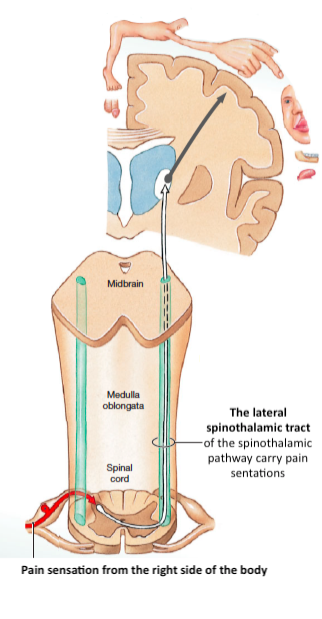
\includegraphics[width=0.7\textwidth]{figures/pathways.png} 
	\caption{Spinothalamic pathway. Modified~\cite{Martini2012}}
	\label{fig:pathways}  
\end{figure}   

Pain is modulated by the descending pathways, where the Periaqueductal Grey (PAG) and the Nucleus Raphe Magnus (NRM) are involved in reducing pain~\cite{Steeds2013}. PAG, also known as anti-nociceptor, is important in the control of pain and surrounds the cerebral aqueduct in Mesencephalon~\cite{Steeds2013}. When this region is electrical stimulated it produces profound analgesia and injection of morphine. PAG receives inputs from the thalamus, hypothalamus, cortex and the spinothalamic tract~\cite{Steeds2013}. Neurons from the PAG region excite the cells in NRM which have a direction towards the spinal cord and block the pain transmission by the dorsal horn cells~\cite{Steeds2013}. Stimulation of NRM produce a strong analgesia and release serotonin which activates the inhibitory interneuron and blocks the pain transmission~\cite{Steeds2013}. The key neurotransmitter is noradrenaline and 5-hydroxytryptamine by modulation pain~\cite{Steeds2013}. 

\subsubsection{Neuropathic pain}
Neuropathic pain is caused by a disorder in the somatosensory system and is often a chronic condition related to injuries or diseases~\cite{Mindruta2013}. The disease occurs at different levels in the nervous system and affects the signaling of pain~\cite{Mindruta2013}. The neuropathic pain would not be described as a single cause or a single specific lesson, but instead, they would be described based on a mechanism~\cite{Mindruta2013}. This mechanism can, however, produce painful symptoms in the same disease, by it would take different aspects~\cite{Mindruta2013}.
The sensation is described as a sudden pain which is burning, tingling, shooting stabbing or numb and can be paroxysmal or continuous. The pain can be divided by the evoked pain into the following:

\begin{itemize}
	\item Hyperalgesia is the pain of abnormal severity followed by a noxious stimulation.
	\item Hyperpathia is an exaggerated and prolonged response to stimulation, which can be delayed in onset and after repeated stimulation. 
	\item Hyperaesthesia is defined as an increased sensitivity to stimulation. 
	\item Allodynia is a painful response to a normally innocuous stimulus. 
	\item Dysaesthesia is an evoked or spontaneous altered sensation is described as a discomfort rather than pain. 
\end{itemize}


It can be difficult to localized the distribution of pain because the distribution is no longer respect by nerves, roots, segments, proximal or distal territories as for nociception pain. However, neuropathic pain can be divided into peripheral, central or mixed syndromes correspond to the anatomy and the underlying disease~\cite{Mindruta2013}. 


\section{Pain measurements}
Pain is described as a complex and subjective experience that poses a number of measurement challenges due to its subjective nature. Nevertheless, pain measurements are necessary for pain studies as well as the evaluation of methods to control pain \cite{libro pain}.
There is no valid and reliable method of objectively quantifying pain at the moment. However, despite the challenges that pain measurement present, several tools and approaches can be employed in order to collect useful pain estimates \cite{pain outcomes paper}. The aim of pain assessment is to diagnose the cause, understand the impact, identify appropriate pain relief strategies and evaluate their effectiveness.\cite{art and science}. There are different dimensions of pain experience that can be assessed: pain intensity, pain affect, pain quality and pain location. Due to the fact that pain is a multidimensional experience, it is needed a multidimensional assessment.


\subsection{Self-reported scales}
Pain cannot be register directly by clinicians, why patient self-report is frequently used to asses the experiences of pain\cite{libro pain}. Within this category it is possible to apply unidimensional and multidimensional scales. However, semi-objective methods such as Pressure Pain Threshold (PPT) can be used by clinicians. 

\subsubsection{Unidimensional scales}
%Maybe make subdivisions i
Unidimensional scales explore only one dimension of pain. The most common assessed dimension of pain is intensity. This could be due to the fact that patients are usually able to provide quantitative pain intensity relatively rapidly \cite{libro pain}. One commonly used unidimensional tool is the Verbal Rating Scales (VRS) which consists of a list of adjectives describing different levels of pain intensity. It is important for an accurate measure using this scale to provide adjectives which reflect the extremes of the dimension, as well as additional adjectives to represent the different levels of pain. Patients are asked to select the word that best describes their level of pain intensity. VRSs are usually scored by listing the adjectives in order of pain severity and assigning each one score as a function of its rank. This type of scales are easy to administer, score and apprehend. However, it has several statistical disadvantages and criticism raised due to the fact that assumes equal intervals between adjectives \cite{libro pain}. For this particular reasons along with others is used when the patient conditions require it \cite{six methods paper}. Other possibility of unidimensional scales is a visual analogue scale (VAS). VAS consists of a 10 cm line, the ends of this line are labeled as the extremes of pain. Patients are asked to indicate the point along the line that best represents the intensity of their pain. The scale is scored by measuring the distance from 'no pain' end to the patient's mark. They are usually measure in millimeters thus, for a 10 cm line gives a high number of response categories. This fact makes the VAS more sensitive to changes in pain intensity. However, one of the drawbacks is that scoring time is higher than for other methods. Numerical Rating Scale (NRS) is also within unidimensional tools of pain intensity measure. NRS consists of asking the patient to rate his or her perceived level of pain intensity on a numerical scale from 0 to 10 (or from 0 to 100), being described 0 as 'no pain' and  10 or 100 equal to 'higest level of pain'. The advantage of NRS is that it not requires patients mobility because the response is given verbally. NRS is a valid method and demonstrate positive and significant correlations with other measures of pain intensity \cite{six methods paper}. Another method is to use pictures or face scales to illustrate facial expressions of different intensities of pain. Even though the primary purpose of this scales were to offer individuals with written language or cognitive difficulties an option to express pain intensity, there is evidence that they are valid methods \cite{libro pain}. 

\subsubsection{Multidimensional scales}
Multidimensional scales are convenient in relentless pain conditions. Multidimensional scales measure several dimensions of pain with different combinations of these dimensions. These scales offer a more detailed reflection of the patient's pain experience \cite{art and science}. Within this category the McGill Pain Questionnaire (MPQ) is used. This method consists of 78 words that describe the pain in sensory, affective and evaluative terms. These tems are arranged in groups acoording to the quality of pain and intensity of this pain. A 6 point VRS is used to determ the intensity of the pain. The MPQ is proved as a valid method support by several studies \cite{libro pain}.  One disadvantage of the MPQ is the length and complexity, why a brief form of this questionnaire has been introduced, the short-form McGill Pain Questionnaire (SF-MPQ). The patients are able to rate the pain with 15 different descriptors in sensory and affective terms. Each descriptor is rated on a 4-point scale. The SF-MPQ includes a VAS for pain intensity as well as a VRS for rating the overall pain experience. Another scale, breif pain inventory (BPI), was developed to assess cancer pain and have been proven as a useful instrument to asses different kinds of pain in several clinical settings \cite{libro pain}. The BPI measures pain severity, pain quality and the disturbance caused in the patients daily life. Two subscale scores pain intensity and pain interference.  


\subsection{Psychophysical methods}
Quantitative sensory testing (QST) evaluates the integrity of the entire sensory neuraxis receptor to the cortex. Even though QST has recieved criticism for being subjective, it is a reliable test. Brain imaging studies provided evidence that subjective pain magnitude scores are associated with objectively measured neural activity in areas of the brain involved in pain processing. QST include different modalities of stimulation, such as thermal, mechanical, electrical, ischemic and chemical. This method provide two different assessments of pain. On the one hand the  evaluation of endogenous pain, which is the pain that the patient experiences due to the disease process. On the other hand, the assessment of induced pain, in order to experiment on pain mechanisms or therapy. \cite{neurop_exam}

%Psycophysics: investigates quantitative the relationship between physical stimuli and the sensations and perceptions they affect.
%Psycophysical methods provide measures for perception and performance. Two approaches thresholds and scaling.

\subsubsection{Measurement of experimental pain}
As a result to a set of experimental noxious stimuli, it is possible to obtain different parameters such as, pain thresholds, tolerance or suprathreshold pain intensities. Threshold is defined as the stimulus that produces an arbitrary, but defined, level of performance. There is a distinction between receptor or absolute threshold and psychophysical or sensory threshold. Absolute threshold is the energy required to elicit response in the primary afferent while the psychophysical or sensory threshold, is the minimal energy necessary to reach perception. Due to the fact that receptor threshold is lower than sensory threshold, the sensory threshold is a convenient parameter which offers the transition point between non-painful and painful stimulus \cite{neurop_exam}.

\subsubsection{Psychophysical Procedure}
Psychophysical research has been mostly concentrated on thresholds measurement owing to, the desire to isolate low-level sensory mechanisms using operationally defined tasks that are intended to minimize the roles of perception and cognition \cite{psy_methods}. There are different procedures in order to measure thresholds.

%Performance-Based Procedures 
%Appearance-Based Procedures

\textbf{Methods of adjustment}
\\
The test subject adjust the magnitude of a stimulus, until a prespecified criterion is reached. This method is commonly used for appearance-based tasks. Currently, this method is not commonly used to obtain performance measures, due to the fact that forced-choice procedures are consider superior. However, the method of adjustment is useful for obtaining a rough threshold estimate to guide the choice of stimulus magnitudes for a forced-choice procedure, when there are different conditions to be measured.

\textbf{Methods of limits} 
\\
In this method, different magnitude stimuli are presented to the test subject, in ascending or descending order. The subject indicates whether or not the stimulus are detected on each presentation. Accordingly, the threshold in each case is the stimulus magnitude at which the response switches from non perception to perception and/or vice versa. The patient's response cannot be evaluated if it is correct or incorrect. \cite{chapter3}. One of the drawbacks of this method  is the observer may get used to reporting that is perceiving a stimulus or not. As a result, he or she  continues to give the same response even at stimulus magnitudes that are higher or lower than the threshold. This phenomena is the error of habituation. Contrarily, the observer may anticipate the response and make a premature judgment, which is call the error of expectation. Another disadvantages using this method is that the parameter value from perception to non-perception differ from non-perception to perception value, due to different artifacts \cite{hysteresis}.

\textbf{Method of constant stimuli}
\\
The stimulus magnitude on each trial is randomly selected from a predefined set. This range is selected to straddle the threshold value. This method generates data, when this data fitted with the appropriate psychometric function, provides the most accurate estimates of the threshold. The choice of this stimulus set sometimes demand pilot work to obtain an estimate of the threshold. The method of adjustment, as explained before, can be useful for this purpose. It is possible to use this method simultaneously with appearance-based procedures. The selection of the stimuli range is crucial. In order to avoid the problem of selecting an incorrect set, an adaptive or staircase procedure is apply.

\textbf{Adaptive or staircase procedure}
\\
An algorithm, that analyzes the previous trials response, selects the stimulus magnitude on each trial. This method can be used simultaneously  with conventional methods as well as with performance-based and appearance-based tasks.

\textbf{Forced-choice Performance Procedures}
\\
Forced-choice tasks can be termed by Alternative Forced-Choice (AFC) or Interval Forced-Choice (IFC). In IFC procedures the stimulus are presented in temporal order. There are different varieties within forced-choice performance procedures, 2AFC procedures are the most popular in psychophysics. In this method, in each trial two stimuli are presented. One of this stimui is the target, which the test subject must select.
